\section{Application to functional neuroimaging}
\label{sec:application}

%%% PURPOSE %%%
The objective of this section is to apply PSA to knowledge discovery in
a practical setting and to assess its ability to
illustrate the decision of the nonlinear and hierarchical classifier trained with real data.
%
We applied the PSA to brain decoding.
%
Because each input is aligned to the standard space (brain),
it is appropriate for the PSA to be applied to brain decoding.
%

%%% Brain decoding %%%
Brain decoding is an act of decoding exogenous and/or endogenous brain states from measurable brain activities \cite{haxby2001distributed,cox2003functional,kamitani2005decoding,shibata2011perceptual,Horikawa2013}.
%
It has been attracting much attention in medical and industrial fields as a major next-generation technology.
%
Possible applications include brain machine interface
(BMI) \cite{laconte2011decoding}, neuro
rehabilitation \cite{sitaram2012acquired} and therapy of mental
disorders \cite{sitaram2007fmri}.
% [Relation with machine learning]
Brain decoding is a function that takes brain activities as input and
brain states as output, and its performance is evaluated by how well it
approximates the real association between these two entities.
%
As such, it falls into the category of machine learning, and it is often
studied in the particular framework of supervised learning \cite{lemm2011introduction}.
%
The brain decoder that well approximates the relationship between brain
activities and brain states might have the knowledge about the brain.
%
Thus, one might consider to extract and visualize the knowledge acquired by the decoder.
%
We do this by applying the PSA to the efficient brain decoder.
% END OF PARAGRAPH

%%% PURPOSE %%%
In order to extract the features common to all human beings,
we trained the decoder as subject-transfer decoder \cite{fazli2009subject,raizada2012makes,marquand2014bayesian}
by a large-scale functional magnetic resonance imaging (fMRI) database.
%
For an ideal subject-transfer decoder, its decoding accuracy does not
deteriorate over the dataset obtained from the population outside the
group of individuals used in its training.
%
To train a better subject-transfer decoder, we will present a
subject-transfer decoder in the form of a neural network with multiple
hidden layers (DNN), a decoder aimed at classifying the brain activities
into seven cognitive task categories.
%
For both training and testing, we used a large open fMRI dataset in Human
Connectome Project (HCP) gathered from over 500 subjects \cite{van2013wu}.
%
In this section, we will show the efficiency of DNN-based decoder
in subject-transfer decoding and thus in capturing
the subject-independent features from big data.

%%% RESULTS %%%
Our subject-transfer decoder achieved higher decoding accuracy than any
other baseline methods like support vector machine (SVM).
%
This is indicative of DNN's superior generalization ability over heterogeneous big data.
%
Also, decoding accuracy improved monotonically as the number of training subjects increased.
%
In the light of the fact that we are engaged in subject-transfer
decoding, this monotonic trend suggests that our training is
successfully extracting more subject-independent features from larger
dataset.
%
In order to extract and visualize these features, we applied PSA to the
trained subject-transfer decoder.
%
By illustrating these features on the map of brain, we were able to find
some connections between these features and functional connectivity
reported in human fMRI studies \cite{raichle2001default,raichle2007default,taylor2009two,cole2013multi}.

%%% OUTLINE %%%
The following sections are structured as follows.
%
In Section\,\ref{sec:fmri_data_specification},
\ref{sec:dnn_as_decoder} and \ref{sec:decoding_setting}, we will provide
the specification of HCP dataset, the summary of our DNN-based decoder
and the evaluation of the subject-transferability, respectively.
%
In Section\,\ref{sec:decoding_accuracy}, we will compare the
performance of our DNN against standard classification techniques, and
show how the decoding accuracy of the DNN improved as the size of the
training dataset increased.
%
In Section\,\ref{PSA_of_dnn_decoder}, the PSMs of the subject-transfer
decoder and its interpretation are summarized.
% END OF PARAGRAPH


\subsection{fMRI data acquisition and preprocessing}
\label{sec:fmri_data_specification}
%%% HCP ABSTRACT %%%
Human Connectome Project (HCP) is a scientific project ``to map macroscopic human brain circuits and their relationship to behavior in a large population of healthy adults'' \cite{van2013wu}, and it provides one of the largest open databases of fMRI that are publically available today.
%
Here, we used the task-evoked fMRI data collected from 499 participants in Quarter 1 through Quarter 6,
which were  preprocessed and registered by \cite{van2013wu,glasser2013minimal} (HCP S500 release).
%
For more details, see the HCP release reference manual\footnote{www.humanconnectome.org/documentation/S500}.
% END OF PARAGRAPH

%%% HCP EXPLANATION  %%%
In this section, we will provide key data specifications and preprocessing procedure.
%
fMRI data of $499$ healthy adults were acquired by a Siemens 3T Skyra, with TR = $720$ ms, TE = $33.1$ ms, flip angle $52^\circ$, FOV = $208 \times 180$ mm, $72$ slices, $2.0 \times 2.0$ mm in plane resolution.
% preprocessing
The preprocessing that had been applied to the fMRI data in the HCP prior to our own modification includes removal of spatial artifacts and distortions, within-subject cross-modal registrations, reduction of the bias field, and alignment to standard space.
% Our preprocessing
In addition to these processes, we applied voxel-wise z-score transformation to the data and averaged the intensity over each anatomical region of interest (aROI).
%
The intention of the latter averaging procedure is to help the decoder learn features that are robust against
large inter-subject variability of brain activities.
%
aROIs were determined by the automated anatomical labeling method \cite{tzourio2002automated}.
%
In the end, the dimension per each preprocessed fMRI scan became 116.
% END OF PARAGRAPH

%%% TASK EXPLANATION %%%
The 499 participants (subjects) in the dataset we studied were asked to perform seven tasks related to the following categories: Emotion, Gambling, Language, Motor, Relational, Social and Working Memory (WM).
%
Each subject performed each task twice with time limits that varies across different tasks (see Table\,\ref{tab:1}).
%
Note that the number of scans conducted in the experiment varies across different tasks.
%
One hundred unrelated subjects completed all seven tasks.
%
The WM class occupied the largest proportion ($20.88$\%) of all scans for each subject.
%
The experimental design of each task is summarized below.
%
See \cite{barch2013function} for more details.
%
%%% Table 1 %%%
\begin{table}[htbp]
 \centering
  \caption{Number of scans per session and its duration (min:sec)}
 {\small
  \begin{tabular}{lccccccc}
   \hline
    & \textbf{Emotion} & \textbf{Gambling} & \textbf{Language} & \textbf{Motor} & \textbf{Relational} & \textbf{Social} & \textbf{WM}\\
   \hline
   Scans & 176 & 253 & 316 & 284 & 232 & 274 & 405  \\
   Duration & 2:16 & 3:12 & 3:57 & 3:34 & 2:56 & 3:27 & 5:01   \\
   \hline
  \end{tabular}
  \label{tab:1}
 }
\end{table}
% END OF TABLE
%
\begin{enumerate}
 \item \textbf{Emotion:} Participants were asked to match one of two simultaneously presented images with a target image (angry face or fearful face). This is a modified version of the emotion task employed in \cite{hariri2002amygdala}.
 \item \textbf{Gambling:} Participants were asked to play a simple game to get money. See \cite{delgado2000tracking} for more details.
 \item \textbf{Language:} After listening to a brief story, participants were asked to answer a two-alternative forced choice question about the topic of the story. See \cite{binder2011mapping} for more details.
 \item \textbf{Motor:} Participants were requested to move one of five body parts (left or right finger, left or right toe, or tongue) as instructed by a visual cue \cite{buckner2011organization}.
 \item \textbf{Relational:} Each participant was presented with two pairs of objects, and was subsequently asked to answer a second-order question regarding the shapes/textures of the objects.
 \item \textbf{Social:} Participants were presented with a movie clip, and were asked to decide whether the movements of the objects in the clips are related with each other in some way. The movie clips were originally prepared by \cite{castelli2000movement} and \cite{wheatley2007understanding}.
 \item \textbf{WM (Working Memory):} Participants were asked to complete two-back working memory tasks and zero-back tasks with four different types of image stimuli (places, tools, faces or body parts).
\end{enumerate}
% END OF SUBSECTION

\subsection{Deep neural networks as decoder}
\label{sec:dnn_as_decoder}
%%% FIGURE 1 %%%
We trained a deep neural network (DNN) with the input being the fMRI
signals over aROIs and the output being their labeled task classes,
i.e., the category of cognitive task performed by the participants.
%
Prior to the training step, all fMRI scans were categorized into seven
task classes, completely disregarding the time order. The weight
parameters of the DNN were then trained to optimize the probability of
successfully classifying the fMRI scans into the seven task categories
(Fig.\,\ref{fig:dnn}).
% END OF PARAGRAPH

The architecture of the trained DNNs are feed-forward neural networks
(see Section \ref{sec:NN}) with one, two and three hidden layers ($n_l = 500$ for any
$l > 0$).
We utilized ReLU for all activation function.
During training,  we adopted a constant learning rate $\eta$, and this
value was set at either of $\{0.1, 1.0\}$ that yielded better result for
the validation dataset (see Section\,\ref{sec:decoding_setting}).
In order to avoid over-fitting, we adopted the dropout technique \cite{Hinton2012}.
Dropout is expected to prevent the decoder from acquiring subject-specific features.
%
\begin{figure}[thpb]
 \begin{center}
  \makebox[\textwidth]{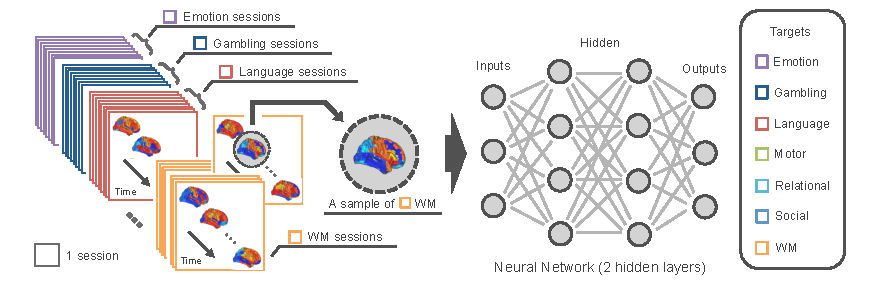
\includegraphics[width=.76\paperwidth]{figures/fig_dnn/fig_dnn.pdf}}
  \caption{\label{fig:dnn}
  We trained DNNs with the input being the fMRI scans and the output being their labeled task classes.}
 \end{center}
\end{figure}
%
% END OF SUBSECTION

\subsection{Subject-transfer decoding}
\label{sec:decoding_setting}
To examine the subject-transferability of our decoder's architecture, we selected hundred individuals from all $499$ subjects who (1) are unrelated with each other and (2) successfully completed all seven cognitive tasks twice.
Let $D$ be the dataset of these $100$ subjects.
We then executed a \textit{leave-10-subjects-out} (or \textit{10-folds}) cross validation to the dataset $D$.
%
To be more specific, the $D$ was partitioned into a test dataset of $10$ subjects, a validation dataset of $10$ subjects, and a training dataset of $80$ subjects without any overlap.
%
We trained our DNN with the training dataset, while using the validation dataset to determine the hyper parameters and to perform early stopping.
%
We then tested the decoding accuracy of trained DNNs over the test dataset.
%
We repeated this cycle $10$ times, choosing different test and validation datasets in each iteration.
%
In order to examine how the size of the dataset influences the decoding
accuracy, we conducted the above experiments with different size of
training dataset ($10, \dots, 80$ and $479$ subjects) without changing the test dataset and the validation dataset.
% with fixing the size of the testing dataset and the validation dataset.
% END OF SUBSECTION

\subsection{Decoding accuracy}
\label{sec:decoding_accuracy}
% Fig. 2
First, we compared the decoding accuracy of the DNNs with those of other baseline methods using the dataset $D$ (see Section\,\ref{sec:decoding_setting}).
% competitors
We trained three neural networks with one, two and three hidden layers, each with the output logistic regression layer.
%
The baseline methods investigated in this study
include logistic (softmax) regression, which corresponds to 0-hidden layer neural network and SVMs with linear kernel and RBF kernel (see Appendix\,\ref{sec:app_baseline_methods} for the specification of these baseline methods).
% result fig
The mean decoding accuracy and its standard deviation in the \textit{leave-10-subjects-out} cross validation are summarized in Table\,\ref{tab:decoding_accuracy}.
%
The decoding accuracies of the DNN decoders not only exceeded the \textit{prior} chance level (the true fraction of the largest class, $20.88$\%), but were also higher than those of the other baseline methods.
%
In particular, the DNN with two hidden layers exhibited the best decoding accuracy of $50.74$\%, which was  significantly higher than that of the RBF-kernel SVM ($p < 0.01 $, one-sided Welch test).
%
Linear methods, the logistic regression and the linear-kernel SVM,
showed poor decoding accuracies that are comparable to the chance level.
%
These results clearly show the advantage of nonlinear decoders over linear decoders in the subject-transfer setting, and suggest that the DNN may be more effective in extracting subject-independent features from big data than the other baseline methods.
% END OF PARAGRAPH
%
%%% Table 1 %%%
\begin{table}
\label{tab:decoding_accuracy}
  \caption{Subject-transfer decoding performance}
 \centering
 \begin{tabular}{lrr}
  \hline
  \textbf{Method} &\textbf{Architecture} & \textbf{Mean accuracy [\%] $\pm$ s.d.} \\
  \hline
  Logistic regression & $116$-$7$ & 20.81 $\pm$ 0.15 \\
  Support vector machine & Linear kernel & 20.87 $\pm$ 0.01 \\
  Support vector machine & RBF kernel & 47.97 $\pm$ 1.57 \\
  Neural network & $116$-$500$-$7$ & 48.94 $\pm$ 1.15 \\
  Neural network & $116$-$500$-$500$-$7$ & \textbf{50.74} $\pm$ 1.25 \\
  Neural network & $116$-$500$-$500$-$500$-$7$ & 50.57 $\pm$ 1.31 \\
  \hline
  % \multicolumn{2}{l}{\textit{Prior} chance level & 20.88} \\ % COMMENT_OUT_IN_AUTHOREA
 \textit{Prior} chance level & & 20.88 \\ % COMMENT_OUT_IN_LATEX
  % \multicolumn{2}{l}{\textit{Prior} chance level \small{(The true fraction of the largest class, WM)} & 20.88 \\ % COMMENT_OUT_IN_AUTHOREA
 % \textit{Prior} chance level {\small (The true fraction of the largest class, WM)} & & 20.88 \\ % COMMENT_OUT_IN_LATEX
  \hline
 \end{tabular}
\end{table}
% END OF TABLE

%%% RESULTS 2 %%%
% purpose
Second, we investigated how the decoder's performance changes with the size of training dataset.
We trained the decoder with various sizes of training dataset, and plotted the decoding accuracy against the dataset size.
% explanation of task
In this set of experiments, we employed the DNN with two hidden layers ($L = 2$),
which showed better decoding accuracy than the $L = 1$ and $L = 3$ versions over the dataset $D$.
% verify using 500 subjects
To evaluate the performance of a DNN decoder trained with a training set of $M$ subjects,
we used the following cross validation procedure.
% dataset explanation
The setup of the cross validation is basically same as the one explained in Section\,\ref{sec:decoding_setting}.
%
At each iteration of the cross validation procedure, we selected $10$ subjects for the test set, $10$ subjects for the validation set, and $M$ subjects for the training set from the dataset $D$ without any overlap.
%
We repeated this process $10$ times, selecting $10$ entirely new subjects for the test set at each iteration.
%
We conducted this set of iteration procedure for $M = 10, \dots, 80$.
%
In order to check the asymptotic trend of the decoding accuracy, we examined the $M = 479$ case as well, in which all of the $499$ subjects registered in the S500 release were used.
% results
The results are displayed in Fig.\,\ref{fig:change_n}.
%% results explanation %%
As the number of subjects in the training dataset increased from $10$ to $80$, the performance of the DNN decoder also increased, as expected.
%
The performance was best at $M = 479$.
%
We attribute this trend to the positive relationship between the size of the training dataset and the reliability of the subject-independent features captured by the DNN decoder.
% END OF PARAGRAPH
%
\begin{figure}[thbp]
\begin{center}
\makebox[\textwidth]{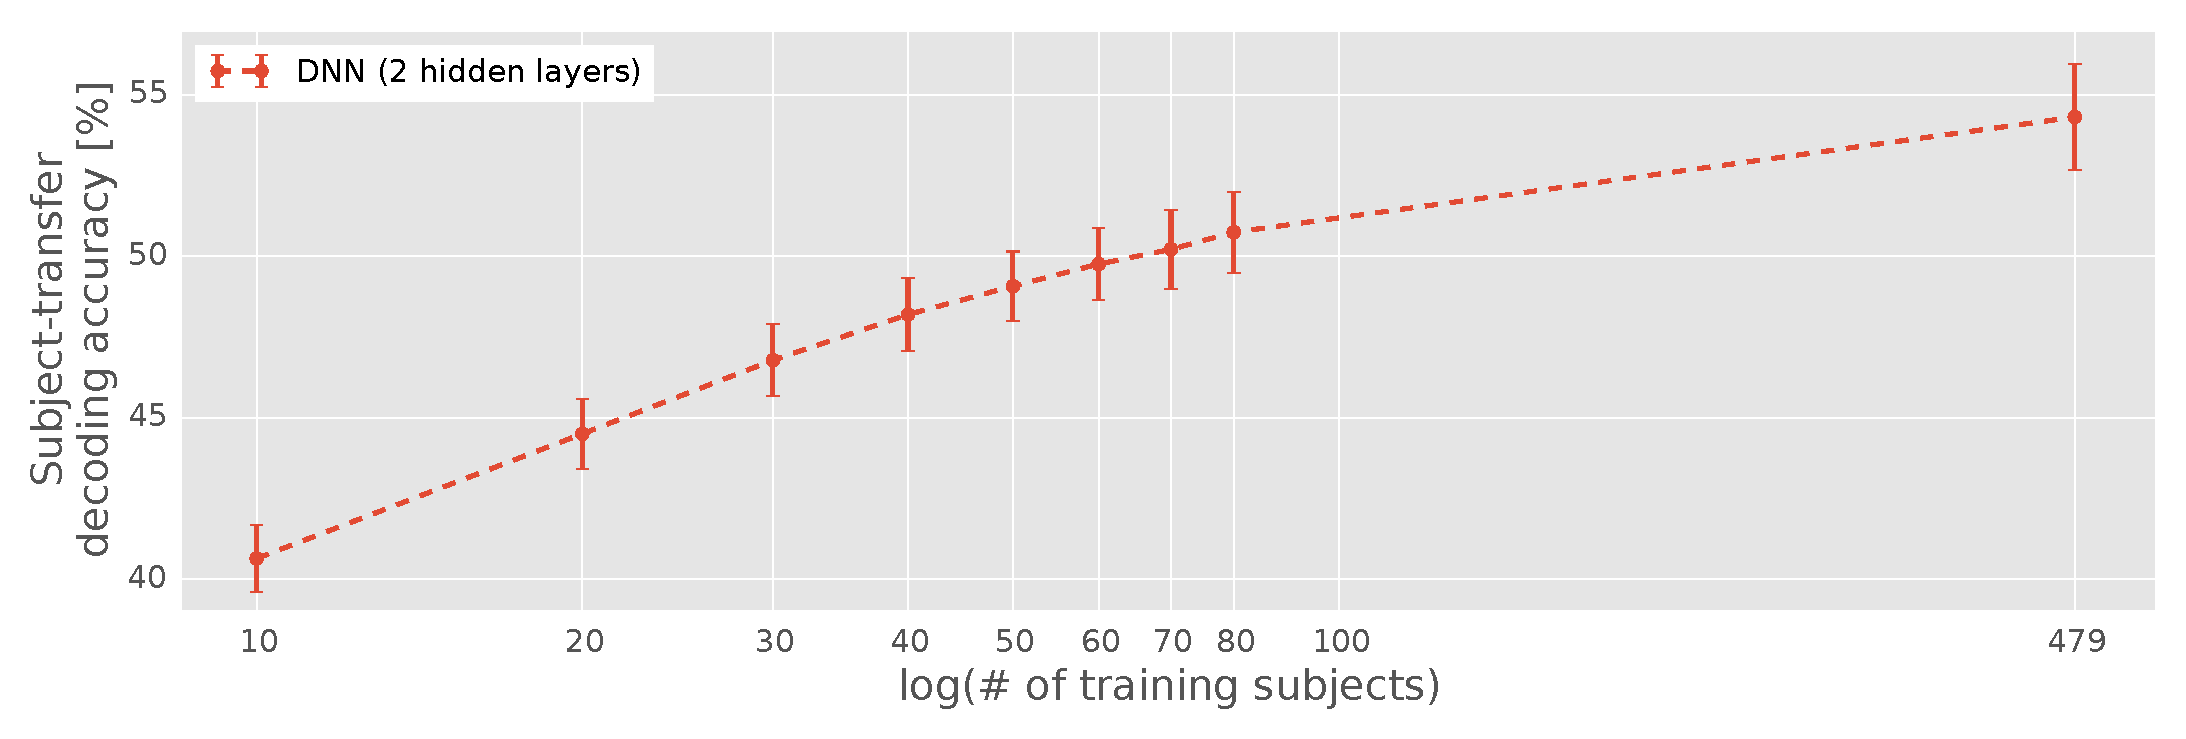
\includegraphics[width=0.73\paperwidth]{figures/fig3/change_n.pdf}}
\caption{\label{fig:change_n}
Mean decoding accuracy plotted against the number of training subjects ($M$) in log scale.
Error bars indicate s.d. across ten cross validation iterations.}
\end{center}
\end{figure}
%

\subsection{PSA of the subject-transfer decoder}
\label{PSA_of_dnn_decoder}
%%% RESULTS 3 %%%
% PURPOSE
In order to extract the discriminative features in brain activities captured by brain decoder trained with the large scale database, we conducted principal sensitivity analysis (PSA).
%
PSA is different from the standard sensitivity analysis in that it quantifies the \textit{combinations} of aROIs used in the decoder's classification, whereas the standard sensitivity analysis computes the independent contribution of each aROI to the decoder's decision.
%
The PSA is more suited for our purpose because there is a strong evidence of functional connectivity among aROIs \cite{Buckner2013, Cole2014}, and classifiers with high decoding accuracy are likely to capture coactivation patterns of aROIs.
% METHODS
The expectation in equation\,\eqref{eq:koyamada_inner_p} depends on the distribution $q$ over the sample space.
%
In order to best approximate the true distribution of $q$, we used the empirical distribution over the dataset of all subjects except the subjects used in $D$.
%% RESULTS
Fig.\,\ref{fig:PSA}(a) shows the first, second an third PSMs for Emotion and Motor classes\footnote{See Appendix\,\ref{sec:app_decoding} for the PSMs of the other classes.}.
%
The set of PSMs presented in Fig.\,\ref{fig:PSA}(a) is one of the $10$ variants of the sets of PSMs obtained in the \textit{leave-$10$-subjects-out} cross validation over the dataset $D$.
%
These variants did not exhibit significant variation.
%
PSMs are superior to standard sensitivity maps in that they can describe the aROIs which act oppositely in characterizing the class.
%
Any pair of anatomical regions with different color assignments in Fig.\,\ref{fig:PSA}(a) contributes to the classifier's decision in opposite direction.
%
Our PSA seems to imply that the information learned by our DNN-based subject-transferable decoder has some correlation with the existing knowledge of functional connectivity supported in neuroscience.
%
For instance,  in the second PSM of Motor class and the first PSM of Social class,
we can identify the two sets of functional connectivity established in previous works, namely fronto-parietal network \cite{cole2013multi} and salience network \cite{taylor2009two}.
%
In the second PSM of Social class, we can also find a component of the default mode network \cite{raichle2007default, raichle2001default} in the left hemisphere.
%
In addition, to quantify the similarity of PSMs, we calculated the
absolute cosine similarity for each pair of the PSMs and aligned the
maps by hierarchical clustering (see Fig.\,\ref{fig:PSA}(b)).
%
For any pair of PSMs ($\bvec{v}_1, \bvec{v}_2$), the absolute cosine similarity was calculated by $\left|\langle\bvec{v}_1, \bvec{v}_2\rangle\right|$, where $\langle\cdot, \cdot\rangle$ is an inner product, because of $\|\bvec{v}\|_2 = 1$ for each PSM $\bvec{v}$.
%
In the similarity matrix, we can confirm two large clusters, consisting mainly of first and second PSMs, respectively.
%
This implies that the functional connectivity interpretation that we
made above for the first and the second PSMs of the Social class and the
the first PSM of the Motor class applies to all the other PSMs sharing
the same cluster memberships (see also Appendix\,\ref{sec:app_decoding}).
%
On the other hand, the sub-principal PSMs, such as the third PSMs of Emotion and Motor classes, showed task-specific features.
%
Finally, note that many of our PSMs span large brain regions.
%
This suggests that the subject independent features that we extracted from the large fMRI database in our deep learning procedure are specific(common) brain-wide networks that activates during particular(all) task(s).
%
\begin{figure}[htpb]
\begin{center}
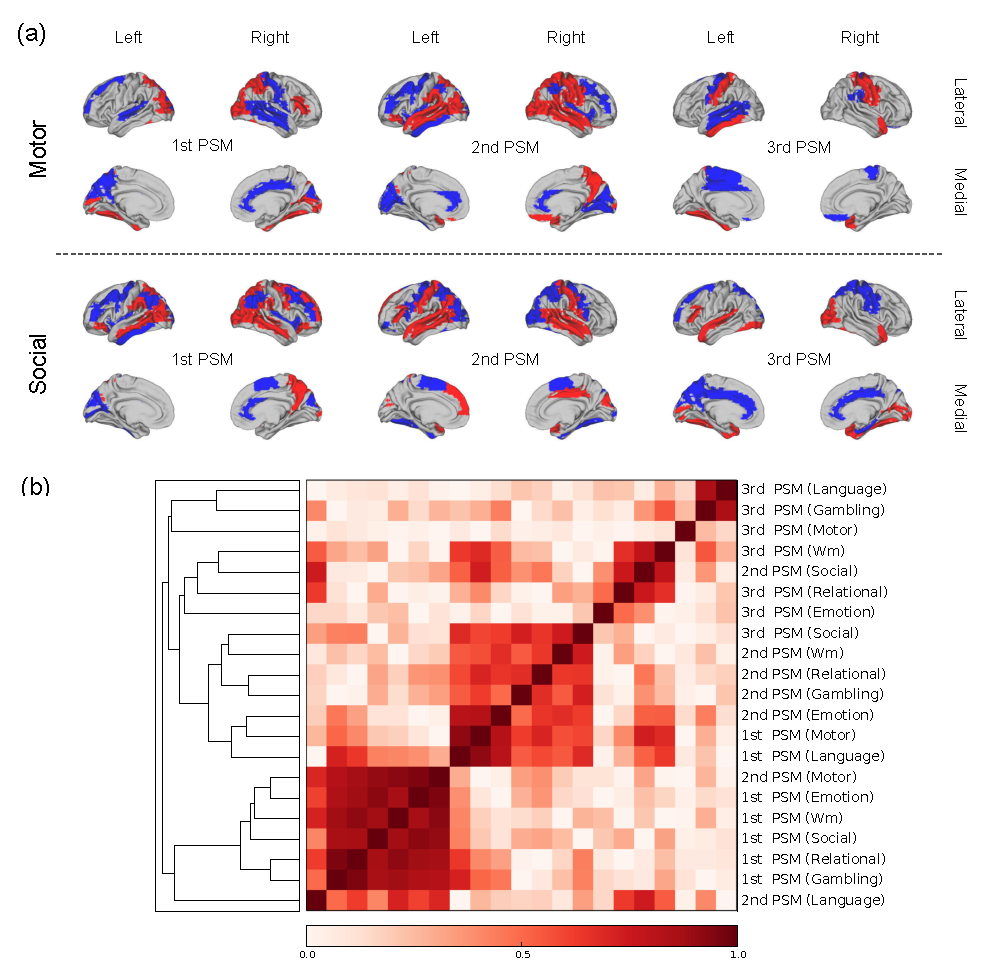
\includegraphics[width=1.\columnwidth]{figures/psa_final/psa_and_similarity.pdf}
\caption{\label{fig:PSA}
(a)
We calculated the first, second and third PSMs for each class. The PSMs
 of Motor and Social classes are shown here (see Appendix\,\ref{sec:app_decoding} for the other classes).
In the visualization of each PSM, we exclusively colored the ROIs with values that are at least one s.d. away from the mean.
Red and blue indicate different signs in the PSM values, i.e., the corresponding aROIs act oppositely in characterizing the class.
(b)
Similarity between maps was evaluated by cosine similarity.
We calculated the absolute value of cosine similarity (for definition,
 see the text) between all pairs of the first, second and third  PSMs of the seven classes. Based on these similarity values, we applied a hierarchical clustering to the set of all the computed PSMs.
The similarity matrix above is based on leaf order in the dendrogram (attached to the left side of the matrix) obtained by the hierarchical clustering. Intensity of the color indicates the degree of similarity.
}
\end{center}
\end{figure}
% END OF SECTION